\documentclass[10pt,a4paper]{book}
\usepackage[utf8]{inputenc}
\usepackage[french]{babel}
\usepackage[T1]{fontenc}
\usepackage{amsmath}
\usepackage{amsfonts}
\usepackage{amssymb}
\author{Hexanome: 4105\\\\Alexis Andra\\Jolan Cornevin\\Mohamed Haidara\\Alexis Papin\\Robin Royer\\Maximilian Schiedermeier\\David Wobrock}
\title{Compte-rendu : Devéloppement Orienté Objet}
\usepackage{graphicx}
\usepackage{xcolor}
\usepackage[hidelinks]{hyperref}
\usepackage{natbib}
\usepackage{listings}
\usepackage{color}
\usepackage{longtable}
\definecolor{lightgray}{rgb}{.95,.95,.95}
\definecolor{darkgray}{rgb}{.4,.4,.4}
\definecolor{purple}{rgb}{0.65, 0.12, 0.82}
\lstdefinelanguage{JavaScript}{
  keywords={typeof, new, true, false, catch, function, return, null, catch, switch, var, if, in, while, do, else, case, break, done, fi, elif, for},
  keywordstyle=\color{blue}\bfseries,
  ndkeywords={class, export, boolean, throw, implements, import, this},
  ndkeywordstyle=\color{darkgray}\bfseries,
  identifierstyle=\color{black},
  sensitive=false,
  comment=[l]{//},
  morecomment=[s]{/*}{*/},
  commentstyle=\color{purple}\ttfamily,
  stringstyle=\color{black}\ttfamily,
  morestring=[b]',
  morestring=[b]"
}
\lstset{
   language=JavaScript,
   frame=single,
   extendedchars=true,
   basicstyle=\footnotesize\ttfamily,
   showstringspaces=false,
   showspaces=false,
   numbers=left,
   numberstyle=\footnotesize,
   numbersep=9pt,
   tabsize=2,
   breaklines=true,
   showtabs=false,
   captionpos=b,
   backgroundcolor=\color{lightgray},
}

\makeindex
\begin{document}
\maketitle
\tableofcontents 
\chapter{Capture et analyse des besoins}
\section{Planning prévisionnel du projet}
Le planning prévisionnel du projet s'est déroulé en trois étapes. Tout d'abord, nous avons identifié les stages nécessaires pour réaliser le projet. Nous avons transformé les missions en tâches réalisables qui sont exprimées par la liste suivante :
\begin{itemize}
	\item{Planning previsionnel du projet (3.0 h)}
	\item{Analyse du modèle (3.0h)}
	\item{Conception du modèle (2.5 h)}
	\item{Analyse des \textit{CU}s, conception des \textit{diagrammes de séquences} (3.5 h)}
	\item{Description textuelle des \textit{CU}s (4.0 h)}
	\item{Implémentation des classes représentant les données dans les fichiers \textit{XMLs} (1.5 h)\footnote{La planification d'une heure et demi peut apparaître insuffisante pour implémenter un modèle. Au moment de la conception de l'architecture, le modèle était considéré comme un ensemble de \textit{JavaBeans}. La réalisation des algorithmes était prévue dans le package contrôleur.}}
	\item{Conception d'IHM (prototype) (8.0 h)}
	\item{Conception d'IHM (précise) (8.0 h)}
	\item{Spécification d'\textit{événements utilisateur} (4.0 h)}
	\item{Conception du diagramme \textit{états-transitions} (6.0h)}
	\item{Implémentation du sérialiseur / désérialiseur (8.0 h)}
	\item{Spécification des interfaces du package contrôleur (5.0 h)}
	\item{Spécification des interfaces du package vue (3.0 h)}
	\item{Spécification des interfaces du package modèle (5.0 h)}
	\item{Conception de diagramme de classes du package contrôleur (6.0 h)}
	\item{Conception de diagramme de classes du package vue (3.0 h)}
	\item{Conception de diagramme de classes du package modèle (6.0 h)}
	\item{Implémentation des observateurs qui notifient la vue (4.0 h)}
	\item{Réalisation de l'IHM (package vue) (20 h)}
	\item{Mock implémentation des classes du package contrôleur (3.5 h)}
	\item{Conception et réalisation des tests unitaires (20 h)}	
	\item{Conception et réalisation des tests fonctionnels (20 h)}
	\item{Implémentation du package contrôleur (30 h)}
	\item{Implémentation du package vue (20 h)}
	\item{Implémentation du package modèle (10 h)}
	\item{Rétro-génération des diagrammes de classes à partir du code (3.0 h)}
	\item{Redaction du glossaire (2.0 h)}
\end{itemize}
~\\Deuxièmement, nous avons essayé de trouver toutes les dépendances entre les missions prévues. Le but de cette démarche était de pouvoir paralléliser au plus les développements. Le graphique suivant montre le déroulement prévisionnel du projet et également qui était le responsable prévu de chaque étape.

\begin{figure}[ht!]
    \centering
    \scalebox{.65}{\input{der.pdf_tex}}
    \caption{Dépendances et déroulement prévisionnel du projet}
\end{figure}

~\\Dans la troisième et dernière étape, nous avons estimé le temps nécessaire pour réaliser ces tâches en utilisant redmine.
\begin{figure}
    \centering
    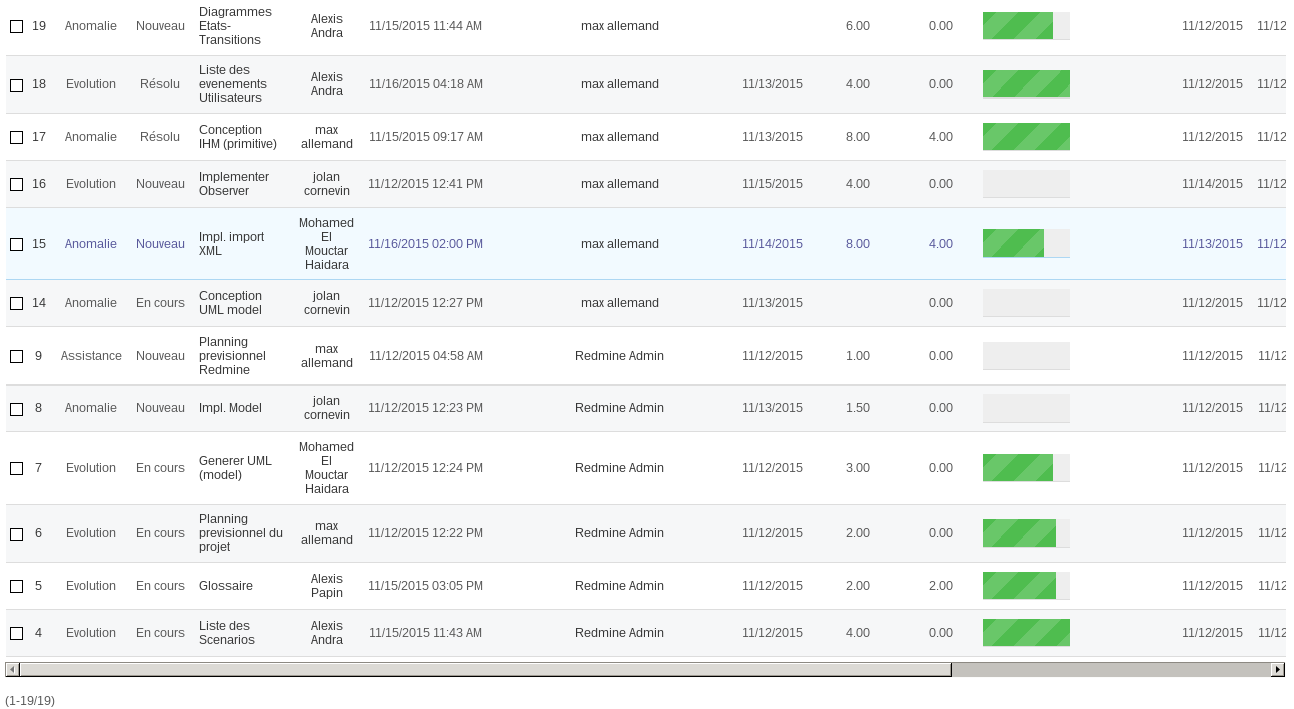
\includegraphics[scale=0.25]{redmine.png}
%http://www.dplot.com/examples/surface-plot-phong-shading.png
    \caption{Capture d'écran de la gestion du projet avec redmine} 
\end{figure}

\section{Modèle du domaine}
\section{Glossaire}
\section{Diagramme de cas d'utilisation}
\section{Description textuelle structurée des cas d'utilisation}
\chapter{Conception}
\section{Liste des événements utilisateur et diagramme états-transitions}
\section{Diagrammes de packages et de classes}
\section{Document expliquant les choix architecturaux et design patterns utilisés}
\section{Diagramme de séquence du calcul de la tournée à partir d'une demande de livraison}
\chapter{Implémentation et tests}
\section{Code du prototype et des tests unitaires}
\section{Documentation JavaDoc du code}
\section{Diagramme de packages et de classes rétro-générés à partir du code}
\chapter{Bilan}
\section{Planning effectif du projet}
Le planning prévisionnel nous a beaucoup aidé dans une réalisation bien pensée ce projet. La connaissance des dépendances entre les modules nous a permi d'éviter qu'un développeur est bloqué et de réaliser les tâches dans le bon ordre.\\
\begin{longtable}{|l|l|r|l|}
\hline
\textbf{Developpeur}&\multicolumn{2}{c|}{\textbf{Tache}}&\textbf{Total}\\
\hline

\hline
Alexis A. & Conception CUs & 4h & 20h\\
\cline{2-3}
& Diagramme état-transition & 4h & ~\\
\cline{2-3}
& Diagramme séquence calcul tournée & 4h & ~\\
\cline{2-3}
& Développement calcul tournée & 8h & ~\\
\hline

\hline
Jolan & Implementation JUnit & 4h & 48h\\
\cline{2-3}
& Implementation du Dijkstra & 25h & ~\\
\cline{2-3}
& Développement modèle & 10 & ~\\
\cline{2-3}
& Conception diagramme modèle & 2h & ~\\
\cline{2-3}
& Conception diagramme séquence & 3h & ~\\
\cline{2-3}
& Correctinos des bugs & 4h & ~\\
\hline

\hline
Mohamed & Conception diagramme modèle & 2h & 57h\\
\cline{2-3}
& Développement Vue & 29h & ~\\
\cline{2-3}
& Développement Contrôleur & 16h & ~\\
\cline{2-3}
& Documentation & 4h & ~\\
\cline{2-3}
& Correction des bugs & 5h & ~\\
\cline{2-3}
& Redaction Design Patterns & 1h & ~\\
\hline

\hline
Alexis P. & Conception CUs & 4h & 20h\\
\cline{2-3}
& Diagramme état-transition & 4h & ~\\
\cline{2-3}
& Diagramme séquence calcul tournée & 4h & ~\\
\cline{2-3}
& Développement calcul tournée & 8h & ~\\
\hline

\hline
Robin & Conception IHM & 6h & 14h\\
\cline{2-3}
& JUnit modèle & 8h & ~\\
\hline

\hline
Max & Planning previsionel & 4h & 71h\\
\cline{2-3}
& Conception architecture et interfaces & 9h & ~\\
\cline{2-3}
& Development Controleur & 18h & ~\\
\cline{2-3}
& Development Modele & 26h & ~\\
\cline{2-3}
& Gestion des taches & 3h & ~\\
\cline{2-3}
& Gestion et réalisation des livrables & 8h & ~\\
\cline{2-3}
& Development JUnit Modele & 3h & ~\\
\hline

\hline
David & Conception CUs & 4h & 52h\\
\cline{2-3}
& Diagramme Sequence & 3h & ~\\
\cline{2-3}
& Développement vue & 20h & ~\\
\cline{2-3}
& Documentation & 8h & ~\\
\cline{2-3}
& JUnit Controleur & 5h & ~\\
\cline{2-3}
& Correction des bugs & 10h & ~\\
\cline{2-3}
& Redaction rapport & 2h & ~\\
\hline
\end{longtable}
~\\Comme le relevé plus haut le montre, le planning prévisionnel était suffisamment précis en ce qui concerne la planification et conception. Par contre, nous n'avons pas réussi à réaliser les implémentations dans le temps prévu. Il y a plusieurs facteurs qui ont contribué à ce retardement. Parmi eux voici les plus importants:
\begin{itemize}
	\item{On était forcé de profondément changer l'architecture dans un moment où la plupart des classes étaient déjà implémentées.}
	\item{Même si pas demandé, nous étions motivés de trouver la meilleure solution possible. Pour ça nous avons parfois implémentés plusieurs alternatives. L'implémentation de l'annulation des commandes est un bon exemple, il sera présenté plus tard dans ce rapport.}
	\item{Les interfaces et classes fournies, qui étaient censées nous simplifier le calcul du chemin optimal, nous ont posés quelques problèmes de compréhension. Il nous était pas évident comment il fallait les utiliser pour en profiter dans le cadre du projet.}
\end{itemize}
\section{Bilan humain et technique}
\subsection{Bilan humain}
Coordonner le projet et notamment distribuer les tâches dans l'équipe était un devoir délicat. D'un côté, un but était la parallélisation des fils de développement. D'autre part, il y avait beaucoup de dépendances entre les étapes prévus. C'est pour ça qu'au début du projet, la priorité était d'identifier une procédure raisonnable qui permettait d'identifier les étapes critiques. Comme je n'ais jamais été en charge d'une équipe aussi nombreuse et puissante je dois admettre que j'avais d'abord sous-estimé ce défi.\\
Le résultat de cet effort nous a bien permis de profiter au maximum des ressources humaines. Néanmoins, il était important de tenir toute l'équipe au courant en ce que regarde les développements effectués en parallèle. En particulier, la convention de bien commenter son code, en combinaison avec une communication fréquente, nous a permis de maîtriser cette mission.\\
Personnellement, je trouvais éprouvant de trouver une bonne granularité pour la distribution des tâches dans l'équipe. Si une charge était trop petite, on risque de perdre du temps en expliquant le contexte. Aurait-elle pu être réalisée plus rapidement directement par la personne qui s'en est déjà occupée ? Sinon, quand les tâches sont trop complexes, on risque qu'un développeur sera bloqué et exclu des événements qui se passent à côté. Comme la section précédente l'a relevé, le nombre d'heures passées sur le projet par développeur n'est pas parfaitement équilibré. Cependant on ne doit pas oublier que les chiffres ne correspondent pas toujours précisément au travail réalisé. Notamment le temps passé sur la planification, communication et réflexion n'est pas facile à mesurer. C'est pour cela qu'il me semble plus avéré d'évaluer l'équipe comme une entité indivisible.\\
Parlant de l'équipe, on peut résumer qu'on était enchanté de pouvoir observer la réalisation de nos conceptions. Même s'il y avait parfois des défis qu'on n'avait pas prévu, l'équipe était toujours motivé pour discuter et trouver la meilleure solution possible.
\subsection{Bilan technique}
Pour réaliser ce projet, nous avons profité d'une grande variété des techniques. Dans le but de permettre à chaque développeur de travailler avec son IDE préféré, nous avons décidé de ne pas garder les fichiers de gestion d'IDE dans le répertoire git. Grâce à cela, nous avons réussi à travailler avec les IDEs \textit{NetBeans}, \textit{Eclipse} et \textit{IntelliJ} en même temps. Concernant les fichiers de conception, nous avons également utilisé plusieurs outils :
\begin{itemize}
	\item{La conception des diagrammes de classes était réalisée avec le logiciel \textit{UMLet} \footnote{http://www.umlet.com/}. Les fichiers utilisés par ce logiciel étaient également partagés dans le répertoire git.}
	\item{Pour tous les autres diagrammes nous avons profité des outils en ligne, particulièrement \textit{Draw.io}, dont une intégration est disponible avec \textit{Google Drive}.}
	\item{Pour automatiquement charger les bibliothèques dont nous avons besoin, nous avons intégré \textit{Apache Maven}. On pourrait argumenter que l'intégration de Maven n'était pas forcement nécessaire, car il y avait seulement quatre dépendances. Néanmoins, son intégration était très confortable pour l'équipe parce qu'on n'a jamais perdu du temps en résolvant les dépendances soulevées par un collègue.}
	\item{Les tests fonctionnels et unitaires étaient réalises en utilisant le framework \textit{JUnit}. Bien que les tests ont grandement contribué à trouver et résoudre des erreurs, nous aurions encore pu intensifier leur intégration. Nous avons suivi le conseil de ne jamais laisser un développeur tester son propre code. C'est en général une bonne pratique, mais nous avons parfois pas établi assez de communication entre un auteur d'une classe et le testeur. Ça peut causer que les tests ne passent pas, car ils n'utilisent pas les interfaces de la manière prévue.}
\end{itemize}
\paragraph{Précisions sur l'implémentation}
Il existe quelques problèmes dont nous sommes conscients et quelques détails que nous souhaitons spécifier ici.
\paragraph{}
Tout d'abord, nous étions très heureux d'avoir pu utiliser JavaFX, le dernier framework de développement de client lourd de Java, bien que les ordinateurs du département n'avaient pas Java 8 d'installé. Nous sommes réjouis de voir que le département fait des efforts pour nous permettre d'utiliser les technologies du moment (JavaFX, Androïd dans le cours d'IHM, ...).
\paragraph{}
Il est possible que lors du redimensionnement de la fenêtre alors que le plan est déjà chargé, il peut problème d'affichage. Ce problème survient essentiellement quand on met la fenêtre en pleine écran directement. De plus, après des agrandissements et des zooms, nous avons remarqué qu'il peut y avoir un décalage entre la position de la souris et la position des intersections sur la partie graphique. Les intersections passent en surbrillance seulement si le curseur est un peu en dessous à droite de la position du rond blanc sur le plan.
\paragraph{}
Pour le patron de conception Etat (\textit{State}), nous avons préféré recréer un objet de l'état correspond à chaque modification, au lieu d'avoir une instance constante (\textit{final}) et statique de chaque état que nous souhaitons réutiliser. Ce choix a été fait car nous voulions avoir un comportement unique à chaque passage dans un état. Ce comportement se situe dans le constructeur de chaque état.
\paragraph{}
Notre patron de conception Commande n'est pas totalement respecté. Dû à des contraintes de temps trop importante et la focalisation sur d'autres fonctionnalités, l'annulation et le rétablissement d'une commande se fait par la restitution du modèle à ce moment. Notre patron Commande est en réalité un mélange entre Commande et Mememto, stockant l'état d'un objet à un certain moment. Pour la copie profonde du modèle, nous n'utilisons pas le patron de conception Prototype, déconseillé par la communauté \footnote{http://stackoverflow.com/questions/64036/how-do-you-make-a-deep-copy-of-an-object-in-java}. Nous sommes conscients que cette manière de faire est beaucoup plus gourmande en mémoire et également en temps processeur. Une amélioration sera vraisemblablement proposée lors du prochain sprint. Afin que la mémoire ne croît pas à l'infini pendant la durée de vie de l'application, nous stockons seulement les dix dernières commandes (copie du modèle du coup) exécutées et les dix dernières annulées.
\paragraph{}
Lors de la création d'une livraison, l'identifiant du client est initialisé à -1.
\paragraph{}
Nous souhaitons, dans un futur proche, améliorer le rapport généré. Celui-ci ne signale pas les retards, ni les attentes endurés par le chauffeur. Il est pour le moment minimaliste. Nous aurions aimé avoir un rapport en HTML avec un peu de style CSS pour avoir un résultat plus attractif.
\paragraph{}
Lors de l'échange de deux livraisons successives, une erreur se produit. Nous n'avons pas eu le temps de corriger ce disfonctionnement de l'application.

\paragraph{}
Finalement, on peut résumer qu'il s'agissait d'un projet complexe et que nous n'avions pas beaucoup de temps pour le réaliser. Nous pensons avoir choisi les bons outils. Ceux-ci nous ont permis d'avancer rapidement et créer un produit fiable.
\appendix{}
\end{document}
\end{document}